\documentclass[11pt]{article}
\usepackage[margin=0.9in]{geometry}
\usepackage{amsmath}
\usepackage{graphicx}
\usepackage{booktabs}
\usepackage{microtype}
\pagestyle{empty}
\setlength{\parskip}{0.4em}

\begin{document}

\begin{center}
{\large\bfseries Branch-wise versus clade-grouped gene-family evolution on the archaeal tree}\\[2pt]
{\small Reconciliation of 7{,}059 gene families on the 257-taxon archaeal species tree, Euryarchaeota root}
\end{center}

\noindent
Reconciling each gene family against the species tree under a duplication--transfer--loss
(DTL) model requires a choice of how finely rates may vary across the tree. We compared two
parameterisations: the \emph{clade-grouped} model, in which all branches of a major clade
share a single set of duplication, loss and transfer rates (and origination weight), and a
\emph{fully branch-wise} model, in which every branch carries its own rates. As a control,
our GPU reconciliation engine reproduces the reference per-family likelihoods to within
Pearson $r=0.999998$, so the comparison reflects the rate model, not the implementation.

Relaxing the clade constraint improves the fit by $\sim$10{,}900 log-likelihood units
(Table~\ref{tab:roots}) while leaving the inferred root unchanged: Euryarchaeota remains the
maximum-likelihood rooting under both models.

A model with thousands of free rates risks describing noise rather than signal, so we tested
it by cross-validation (Figure~\ref{fig:cv}). We estimated the rates from one half of the gene
families and used them to predict the likelihood of the other half, which took no part in
fitting. The branch-wise model predicts these withheld families better than the clade-grouped
model, by $+0.44$ log-likelihood units per family --- in the same direction, though smaller,
as on the families used for fitting ($+2.71$ per family). Had the additional parameters been
absorbing noise they would have \emph{degraded} prediction on the withheld families; instead
they improve it. The among-branch rate variation the model adds is therefore real, not an
artefact of over-parameterisation.

That variation has a clear and interpretable structure (Figure~\ref{fig:rates}). Duplication
and transfer rates are essentially \emph{clade-constant}: within each named clade the
per-branch estimates scarcely depart from a single value (clade membership explains
$R^2\!\approx\!0.94$ of their variance). Loss is markedly less clade-structured
($R^2\!\approx\!0.38$): its extra variation is distributed across branches rather than captured
by clade identity. Biologically, gene gain (duplication, transfer) is well summarised by one
rate per clade, whereas gene loss is more branch-idiosyncratic.

The reconstructed ancestral genome is robust to this added flexibility
(Figure~\ref{fig:laca}). Of the 7{,}059 families, the branch-wise model assigns 903 to the
last archaeal common ancestor and the clade-grouped model 772; 722 are common to both (Jaccard
$0.76$), and the per-family probabilities of origination at the root agree closely
($r=0.96$). The two models therefore recover essentially the same ancestral gene set, the
branch-wise model reconstructing a modestly larger genome.

\begin{table}[h]
\centering\small
\begin{tabular}{lrrcc}
\toprule
 & \multicolumn{2}{c}{branch-wise model} & branch-wise & clade-grouped \\
candidate root & $\log L$ (nats) & $\Delta$ & AU & AU \\
\midrule
Euryarchaeota    & $-1{,}631{,}537$ & $0$         & $\mathbf{0.63}$ & $\mathbf{0.64}$ \\
HalobacThermopl  & $-1{,}635{,}105$ & $-3{,}568$  & 0.00 & $<$0.05 \\
TackA            & $-1{,}635{,}514$ & $-3{,}977$  & 0.00 & $<$0.05 \\
MHH              & $-1{,}637{,}704$ & $-6{,}167$  & 0.00 & $\mathbf{0.49}$ \\
Kor              & $-1{,}637{,}909$ & $-6{,}372$  & 0.00 & $<$0.05 \\
TACA             & $-1{,}638{,}428$ & $-6{,}891$  & 0.00 & $<$0.05 \\
DPANN            & $-1{,}639{,}707$ & $-8{,}170$  & 0.00 & $<$0.05 \\
TAC              & $-1{,}639{,}970$ & $-8{,}433$  & 0.00 & $<$0.05 \\
Asgard           & $-1{,}641{,}098$ & $-9{,}561$  & 0.00 & $<$0.05 \\
MicraDia         & $-1{,}642{,}346$ & $-10{,}809$ & 0.00 & $<$0.05 \\
AMD              & $-1{,}642{,}470$ & $-10{,}933$ & 0.00 & $<$0.05 \\
UndineClu2       & $-1{,}643{,}241$ & $-11{,}704$ & 0.00 & $<$0.05 \\
Alti             & $-1{,}643{,}347$ & $-11{,}810$ & 0.00 & $<$0.05 \\
Cluster2         & $-1{,}643{,}727$ & $-12{,}190$ & 0.00 & $<$0.05 \\
Micra5           & $-1{,}644{,}060$ & $-12{,}523$ & 0.00 & $<$0.05 \\
\bottomrule
\end{tabular}
\caption{All 15 candidate roots: branch-wise log-likelihoods (per-branch model), their
difference from the best, and the approximately-unbiased (AU) support under the branch-wise
model and under the parsimonious clade-grouped model. Both models place Euryarchaeota first.
The clade-grouped model additionally retains MHH (AU 0.49) --- the \{Euryarchaeota, MHH\}
region --- whereas the branch-wise model separates the roots strongly and supports
Euryarchaeota alone; we read the latter's sharpness as model richness, not stronger evidence.
Whole-dataset fit: clade-grouped $-1{,}642{,}425$ vs branch-wise $-1{,}631{,}537$
($+10{,}888$; held-out cross-validation $+1{,}556$, not overfitting; Figure~\ref{fig:cv}). AU
values are scale-invariant bootstrap supports; the listed branch-wise $\log L$ are on
gpurec's marginal-likelihood scale.}
\label{tab:roots}
\end{table}

\begin{figure}[h]\centering
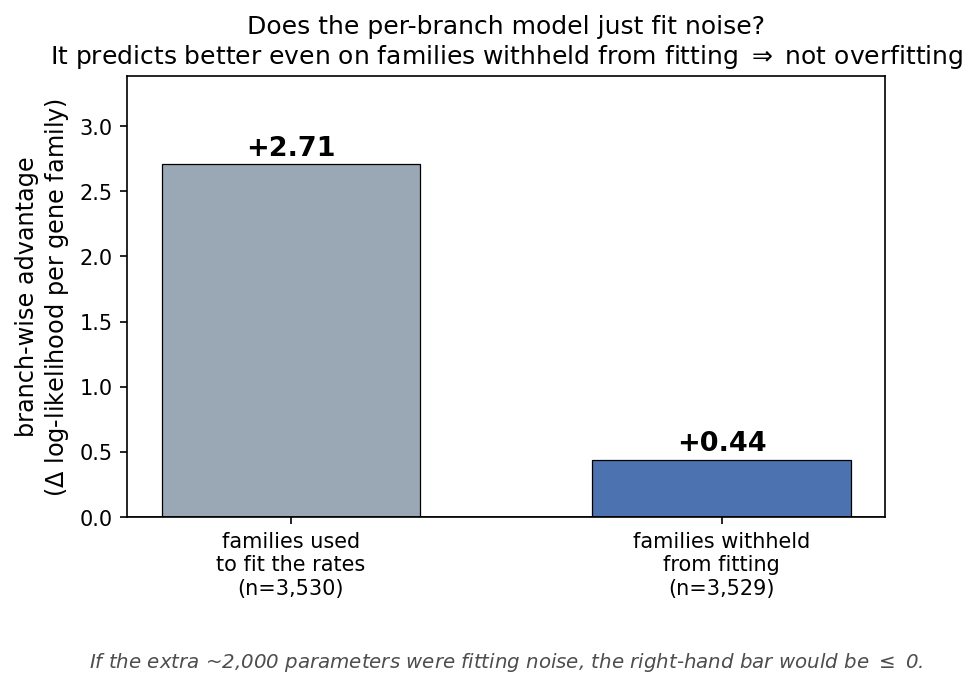
\includegraphics[width=0.5\textwidth]{cv_overfit_bigtree_Eury.png}
\caption{Cross-validation against over-parameterisation. The branch-wise model's predictive
advantage over the clade-grouped model, per gene family, on families used to fit the rates
versus families withheld from fitting. Both are positive --- the per-branch model predicts the
withheld families better --- so the added rates are real signal. Had they been fitting noise,
the right-hand bar would be $\le 0$.}
\label{fig:cv}
\end{figure}

\begin{figure}[h]\centering
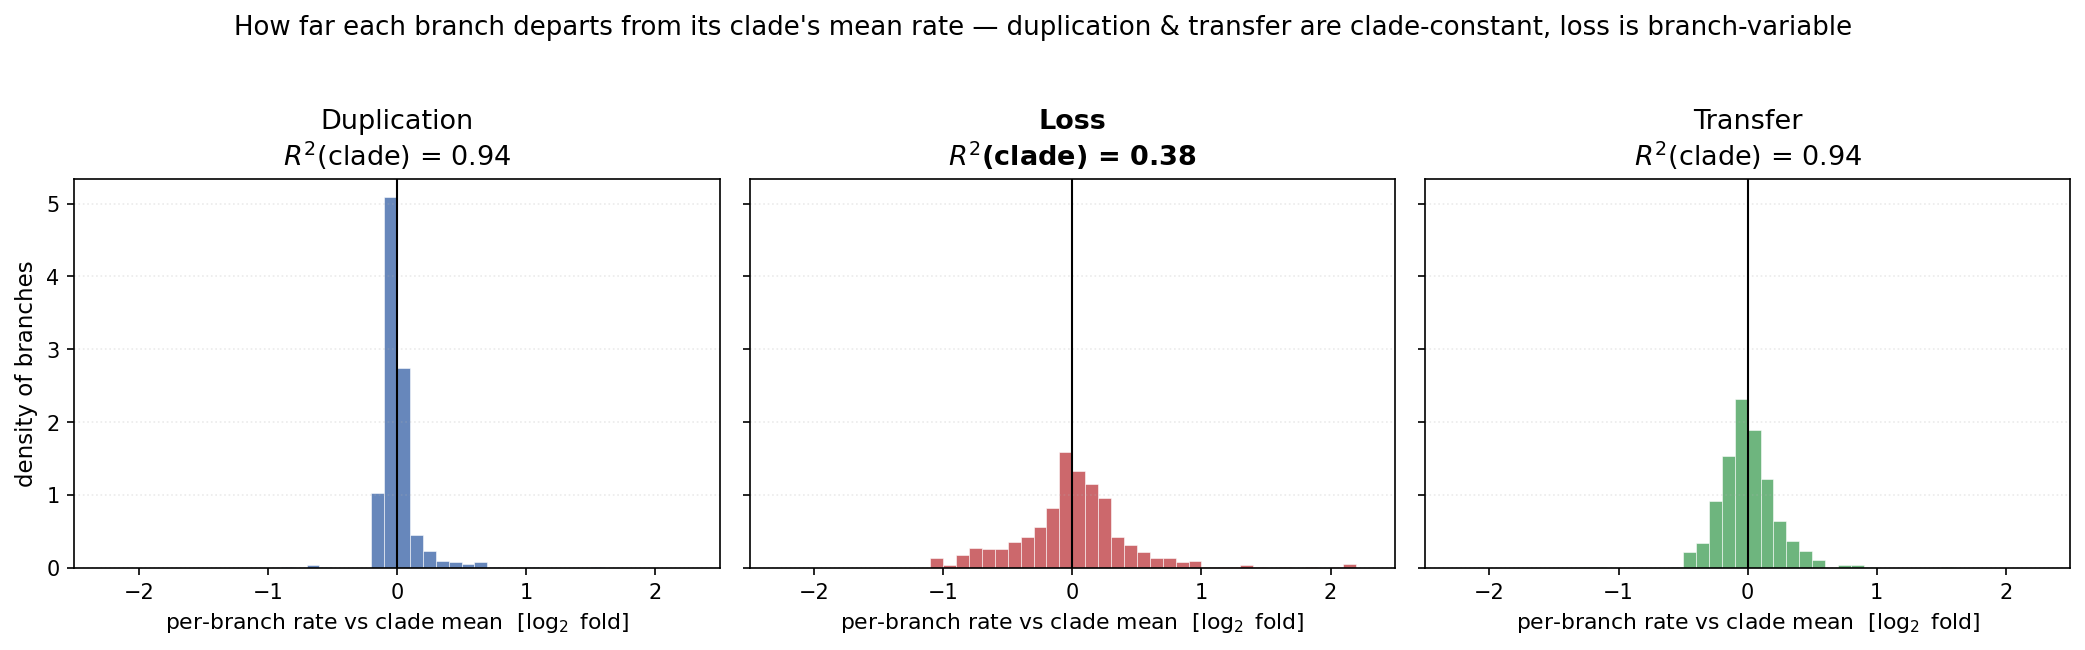
\includegraphics[width=0.98\textwidth]{rate_deviation3_bigtree_Eury.png}
\caption{Departure of each branch's fitted rate from its clade's mean rate ($\log_2$ fold;
shared axes). Duplication and transfer form a sharp spike at zero --- the per-branch
estimates scarcely leave their clade mean, so clade membership explains $R^2\!\approx\!0.94$
of the variance --- whereas loss is broad ($R^2\!\approx\!0.38$), i.e.\ branch-specific. Gene
gain (duplication, transfer) is well summarised by one rate per clade; gene loss is not.}
\label{fig:rates}
\end{figure}

\begin{figure}[h]\centering
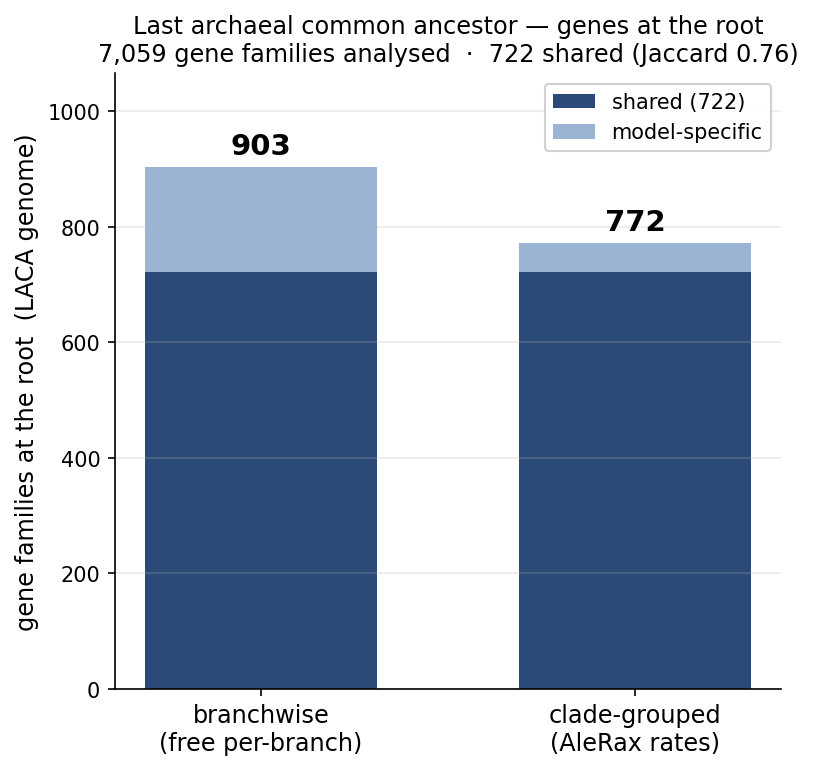
\includegraphics[width=0.5\textwidth]{laca_families_bigtree_Eury.png}
\caption{Reconstructed last archaeal common ancestor (LACA) gene content: 903 families under
the branch-wise model vs.\ 772 under clade-grouped rates, 722 shared (Jaccard 0.76), of 7{,}059
analysed.}
\label{fig:laca}
\end{figure}

\end{document}
